% CFP and link to instructions for authors:
% http://www.iscb.org/ismb2014-submission/1765-ismb2014-call-for-proceedings
\documentclass{bioinfo}
\copyrightyear{2014}
\pubyear{2014}
\usepackage{url}

\newcommand{\todo}[1]{\footnote{\textbf{TODO:} #1}}
 
\begin{document}
\firstpage{1}

\title[ADAM: Cloud Scale Genomic Processing]{ADAM: A Data Format And Pipeline For Cloud Scale Genomic Processing}
\author[Massie and Nothaft \textit{et~al}]{Matt~Massie\,$^{1,\dagger,}$\footnote{These authors contributed equally.} , Frank~Austin~Nothaft\,$^{1,\dagger, *}$,
Christopher~Hartl\,$^{2}$, Christos~Kozanitis\,$^1$, Andr\'{e}~Schumacher\,$^3$, Timothy~Danford\,$^4$, Carl~Yeksigian\,$^4$, Jey~Kottalam\,$^1$,
Arun~Ahuja\,$^5$, Neal~Sidhwaney\,$^5$, Jeff~Hammerbacher\,$^5$, Michael Linderman\,$^5$, Anthony~D.~Joseph\,$^1$, and David~Patterson$\,^{1,}$\footnote{To whom
correspondence should be addressed.}}
\address{$^{1}$Department of Electrical Engineering and Computer Science, University of California, Berkeley, CA\\
$^{2}$The Broad Institute of MIT and Harvard, Cambridge, MA\\
$^{3}$International Computer Science Institute (ICSI), University of California, Berkeley, CA\\
$^{4}$GenomeBridge, Cambridge, MA\\
$^{5}$Carl Icahn School of Medicine at Mount Sinai, New York, NY}

\history{Received on XXXXX; revised on XXXXX; accepted on XXXXX}

\editor{Associate Editor: XXXXXXX}

\maketitle

\begin{abstract}

\section{Motivation:}
By using cloud computing services or large computing clusters to process genomic data, we can significantly decrease the cost and latency of genomic analysis. However,
current genomics data formats and processing pipelines were introduced prior to many significant advances in cloud and cluster computing technologies. Through the careful
design of new file formats, we can unlock the advantages of distributed computing and also ensure that the file formats can easily be optimized for future computing advances.

\section{Results:} We introduce ADAM, a set of file formats and command line tools for processing genome data on clusters and in the cloud. On a high coverage~(60$\times$)
250GB NA12878 BAM file, with ADAM we are able to perform Sorting and Duplicate Marking in under 50 minutes on a 100 node cloud-based cluster~(a 50$\times$
performance improvement). On a single node, our tools performs twice as fast as Picard and SAMtools, at half the cost. ADAM files are up to 25\% smaller than equivalent
compressed BAM files.

\section{Availability:}
The ADAM project website is at \url{http://adam.cs.berkeley.edu}. ADAM is open source under the Apache 2 license, is deployed through Maven,
and the source is available through GitHub.

\section{Contact:} \href{massie@berkeley.edu}{\{massie,fnothaft,pattrsn\}@berkeley.edu}
\end{abstract}

\section{Introduction}
\label{sec:introduction}

As noted by \citet{mcpherson09}, the improvement of next generation sequencing~(NGS) methods has made data processing a bottleneck. This impediment has significant
impact on scientists who are using genomics in a time-sensitive clinical setting, or who are working on very large datasets~(e.g., for genome wide association studies, GWAS,
see~\citet{wang05}). The Sequence/Binary Alignment/Map~(SAM/BAM) and Variant Call Format~(VCF) file formats were designed before multi-node processing and cloud
computing were in vogue, and were optimized for single node processing~\citep{li09}. However, the past five years have seen significant improvements in both hardware
and software for distributed computing~\citep{barroso13}.

Distributed processing can improve both the cost and latency of genomic processing. However, there are scalability limitations inherent to the BAM and VCF file formats that limit
the performance improvements seen by distributing data over more than 8 nodes. This limitation is seen in \citet{niemenmaa12} and is discussed in
more detail in ~\S\ref{sec:approach}. We choose to rethink file formats for genomics to unlock the advantages of distributed computing platforms, and to enable easy adjustment
to future computing trends. We are guided by the following design goals:

\begin{itemize}
\item Many genomics applications only access selective portions of data~(certain groups of records, or fields within records). Our new formats should support these access
patterns when used as a flat file, and also when used as a database.
\item Scientists collectively want to process data in several different programming languages. To avoid incompatibilities, it is important that our new formats are natively
supported across many programming languages.
\item Genomic data will be processed on various computing systems, including single workstations, large dedicated clusters,
and using cloud computing services. We must jointly optimize for these diverse platforms.
\item The file formats we use must be flexible enough to support new fields, but should be straightforward to manage and maintain.
\end{itemize}

To address these problems, we introduce ADAM, a set of formats, application programming interfaces~(APIs), and processing stage implementations for genomic data.
ADAM is fully open source under the Apache 2 license, and is implemented on top of Avro~\citep{avro} and Parquet~\citep{parquet} for data storage. Our reference pipeline
is implemented on top of Spark, a high performance in-memory Map-Reduce system~\citep{zaharia10}. This combination provides an explicit data schema, enables
natively compatible file access across many programming languages, improves the scalability of distributed applications, and reduces the disk I/O bottleneck faced by many
contemporary genomics applications. These changes lead to significant performance improvements, and improve the format's cross-platform portability. On a single
node, we are able to speedup sort and duplicate marking by 2$\times$. More importantly, on a 250 Gigabyte~(GB) high~(60$\times$) coverage
human genome, this system achieves a 50$\times$ speedup on a 100 node computing cluster, fulfilling the promise of scalability of ADAM.
We provide an extensive review of ADAM's performance in~\S\ref{sec:performance}.

The ADAM format provides explicit schemas for read and reference oriented~(pileup) sequence data, variants, and genotypes. The schemas are implemented in Apache
Avro, a cross-platform/language serialization format. It provides native access to ADAM data across languages, without requiring the development of APIs or libraries.
This approach eliminates the possibility of library incompatibilities and reduces the likelihood of programming errors. Additionally, any application that implements the
ADAM schema is compatible with ADAM, which allows for a greater variety of access patterns and programming models to be built on top of ADAM. The ADAM stack is inspired
by the ``narrow waist'' of the Internet Protocol~(IP) suite (see Figure~\ref{fig:stack-model}). We consider this stack model to be the greatest contribution of ADAM, as it ensures
that the basic ADAM file formats can easily be optimized for new computing technologies. While the base abstraction provided by ADAM focuses on the syntax of data
interchange, the stack design allows for semantics that better represent the biology to be implemented on ADAM.

In this paper, we introduce our new approach in~\S\ref{sec:approach}, and explain the benefits it provides. We review the design and performance of our pipeline
in~\S\ref{sec:methods}. Finally, we provide a comprehensive comparison of ADAM against other data formats and discuss the future growth of ADAM in~\S\ref{sec:discussion}.

\section{Approach}
\label{sec:approach}

As we noted in the introduction, instead of trying to extend the BAM and VCF file formats, we choose to re-imagine these formats. Despite several attempts to adapt the
BAM and VCF file formats for distributed processing~\citep[see][]{niemenmaa12}, they have been limited in their ability to scale to larger cluster sizes due to several issues
intrinsic to BAM and VCF:

\begin{itemize}
\item BAM and VCF both depend on centralized headers, which must be globally distributed; and
\item BAM and VCF both have irregular record sizes, which limits the efficiency of row-parallel reading. 
\end{itemize}

These characteristics limit the performance of applications that desire parallel access to all records of a BAM or VCF file. However, this points at another problem: traditional
flat file formats are not ideal for genomics. Traditional flat file formats do not provide:

\begin{itemize}
\item \textbf{Database Queries:} Extending BAM to support standard database queries required a significant extension~\citep{kozanitis13}.
No such extension exists for VCF data.
\item \textbf{Efficient Predication:} Typically, a user would only like to process a subset of records. Currently, for both BAM and VCF, a user must load all
records and then perform a filter, which is inefficient. BAM supports the inclusion of an index file~(BAM Index, BAI), but this index file can only accelerate
reference position-based filtering patterns\footnote{Typically, the first step of variant calling involves a filter that removes low quality reads. These filters
are based on position-independent data~(e.g. mapping quality, Boolean flags) and cannot be accelerated with the BAI.}.
\item \textbf{Projection of Specific Fields:} It is typical for an application to only read some fields of a BAM record across all records, especially for
statistics collection tools like SAMtools' \texttt{flagstat}~\citep{li09}. Row-oriented formats like BAM and VCF cannot support these access patterns.
\end{itemize}

Moving forward, we seek to meet two major goals: we want to provide an extensible architecture that will allow for efficient future extension of the
file format, and we want to provide an initial implementation of that architecture that addresses the problems introduced above. In the remainder
of this section, we review our high-level architecture that provides extensibility, and then we provide a technical overview of our reference pipeline.

\subsection{Architectural Overview}
\label{sec:architectural-overview}

Our primary criticisms of BAM and VCF are that the formats are difficult to specialize for certain processing patterns without
changing the implementation of the formats themselves. This issue is similar to the problems addressed during the development of the Open
Systems Interconnection~(OSI) model and Internet Protocol~(IP) stack for networking services~\citep{zimmermann80}. The developers
of the OSI model and the IP stack needed to make many different technologies and systems function in unison---to do this, they introduced the
concept of a ``narrow waist,'' which guaranteed that a new protocol or technology would be compatible with the rest of the system if it implemented
one specific interface.

We draw inspiration from the development of networking standards---we believe that our largest contribution is the explicit ADAM schema, which is the ``narrow waist''
in our stack. This schema allows components to be cleanly interchanged as long as they implement the ADAM schema. Figure~\ref{fig:stack-model} shows our stack.

\begin{figure}[h]
\begin{center}
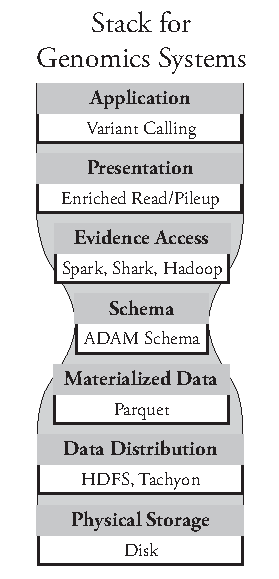
\includegraphics[width=0.4\linewidth]{stack-model.pdf}
\end{center}
\caption{A Stack Model for Genomics}
\label{fig:stack-model}
\end{figure}

The seven layers of our stack model are decomposed as follows, traditionally numbered from bottom to top:

\begin{enumerate}
\item {\bf Physical Storage:} This layer coordinates data writes to physical media, usually magnetic disk.
\item {\bf Data Distribution:} This layer manages access, replication, and distribution of the genomics files that have been written to disk.
\item {\bf Materialized Data:} This layer encodes the patterns for how data is encoded and stored. This provides read/write efficiency
and compression.
\item {\bf Data Schema:} This layer specifies the representation of data when it is accessed, and forms the narrow waist of the pipeline.
\item {\bf Evidence Access:} This layer implements efficient methods for performing common access patterns such as random database
queries, or sequential/parallel reading of records from a flat file.
\item {\bf Presentation:} The presentation layer provides the application developer with efficient and
straightforward methods for querying the characteristics of individual portions of genetic data.
\item {\bf Application:} Applications like variant calling and alignment are implemented in this layer.
\end{enumerate}

The ADAM schema is represented using Apache Avro~\citep{avro}, an open-source, cross-platform data serialization framework similar
to Apache Thrift and Google's Protocol Buffers~\citep{thrift, protobuf}. Avro was chosen as the interchange format for several reasons:

\begin{itemize}
\item Avro is an open-source framework covered by the Apache 2 license, which means that Avro can be used with both open and closed source software.
\item Avro has broad cross-platform support. Natively, Avro supports C/C++/C\#, Java, Scala, Python, Ruby, and php.
\item Avro provides a clear and human readable language for explicitly describing the schema of an object~(Avro Description Language, AVDL).
\item Avro is natively supported by several common Map-Reduce frameworks and database systems.
\item Avro schemas can be updated without breaking compatibility with objects written using a previous version of the schema.
\end{itemize}

For a system to implement the ADAM format, it must read/write ADAM objects that are defined by Avro schemas. As such the schemas
provide the common ground for tools to interoperate, thereby allowing the user to interchange one tool for another and minimize
tool or vendor lock-in.

A well defined software stack has several other significant advantages. By limiting application interactions with layers lower than the presentation layer,
application developers are given a clear and consistent view of the data they are processing, and this view of the data is independent of whether the data
is local or distributed across a cluster or cloud. By separating the API from the data access layer, we unlock significant flexibility. With careful design in the data
format and data access layers, we can seamlessly support conventional flat file access patterns, while also allowing easy access to data with database methods.
By treating the compute substrate and storage as separate layers, we also drastically increase the portability of the APIs that we implement.

\subsection{Reference Implementation}
\label{sec:reference-implementation}

We present a reference implementation of a read processing pipeline~(\texttt{adam-core}). This implementation is fully open source
and is designed for a distributed, in-memory Map-Reduce framework. We do not optimize for a specific computing platform---rather, we have designed
agnostically for commodity clusters and for cloud computing platforms. We discuss this decision in~\S\ref{sec:single-vs-clusters-vs-cloud}. Our reference
implementation provides several read processing stages that can be either run from a command line, or executed by another application through
an API, as well as an API for enriched datatypes. These APIs are similar to those provided by SAMtools~\citep{li09} and Picard~\citep{picard}.

As mentioned in~\S\ref{sec:introduction}, we built our system using the Avro data serialization format, the Parquet columnar store, and the Spark Map-Reduce
framework~\citep{avro, parquet, zaharia10}. We have already explained the reason for using Avro, we now give the rationale for using Spark and Parquet.

\paragraph{Spark, In-Memory Map-Reduce:}
\label{sec:spark}

Apache Spark is an in-memory, distributed Map-Reduce framework that was introduced in \citet{zaharia10} and further described in \citet{zaharia12}.
Although it is compatible with the Hadoop~\citep{hadoop} ecosystem, Spark differs from conventional implementations of the Map-Reduce framework
originally proposed by Google in \citet{dean08}, since it avoids writing data to disk whenever possible and instead caches
data in memory. This optimization provides a dramatic speedup for iterative computations---Spark sees a 30--100$\times$ speedup on iterative jobs by eliminating
disk I/O and by improving resource utilization by pipelining computation. This pattern is a good fit for genomics because:

\begin{itemize}
\item With the increasing size of genomic datasets, disk I/O is a bottleneck for modern genomics systems. By persisting data in memory between processing stages,
we are able to lessen the disk I/O penalty and improve latency.
\item Many genomic processing stages are iterative. For many applications, iteration implies that stages can be pipelined, which improves system performance on large
parallel systems\footnote{Performance is improved as pipelining reduces the number of executors that become idle at the start and end of stages by overlapping the
two stages.}.
\item Additionally, memory cost and capacity is improving very quickly. Datacenters are moving towards a model where large ``clouds'' of memory are replacing
storage~\citep{barroso13}.
\end{itemize}

An additional benefit of Spark is that its programming interface supports Java, Scala, and Python\footnote{A programming interface for the R programming language will
be available in the first half of 2014.}.

\paragraph{Parquet, Columnar File Format:}
\label{sec:parquet}

Parquet is a columnar file format that is designed for distributed computing. Columnar stores differ from conventional file formats as they group data together
by field instead of by record. This orientation enables very high read performance, improved compression~\citep[see][]{abadi06}, and the efficient serialization of a subset
of fields. Parquet has other benefits:

\begin{itemize}
\item Parquet operates by splitting a single dataset into many smaller files that contain \emph{row groups}\footnote{In Parquet, a \emph{row group} contains a subset
of rows of data from the dataset. The row groups are then stored in columnar format.}. This division enables both parallelism by column and by row which increases read
parallelism.
\item Parquet provides \emph{predicate pushdown}, where user defined filters are applied while records are being read. This feature can lead to a $>$2$\times$ performance increase.
A detailed analysis of Parquet's predicate pushdown functions for genomics applications can be found in \citet{massie13}.
\end{itemize}

Figure~\ref{fig:file-format} shows how ADAM in Parquet compares to BAM. We remove the file header from BAM, and distribute these values across all of the stored
records. This dissemination eliminates global information and makes the file simple to distribute across machines. This distribution is effectively free in a columnar store,
as the store just notes that the information is replicated across many reads.

\begin{figure}[h]
\begin{center}
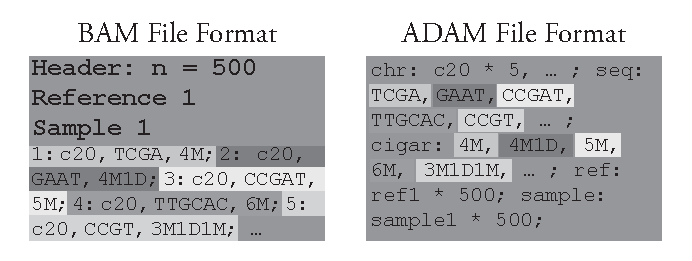
\includegraphics[width=\linewidth]{file-format.pdf}
\end{center}
\caption{Comparative Visualization of BAM and ADAM File Formats}
\label{fig:file-format}
\end{figure}

Our reference pipeline implementation provides two components:

\begin{itemize}
\item \texttt{adam-cli}, a command line toolkit for converting data to/from the ADAM format, and for performing transformations, and
\item \texttt{adam-core}, an API for processing genomic data that is stored in the ADAM format and is contained in memory.
\end{itemize}

\noindent We further describe the functionality provided by the command line toolkit and the API in~\S\ref{sec:data-transformations}.

\section{Methods}
\label{sec:methods}

ADAM contains formats for storing read and reference oriented sequence information, and variant/genotype data. The read oriented sequence format is both forward and
backward compatible with BAM/SAM, and the variant/genotype data is forward and backward compatible with VCF. In this section, we discuss the specific data formats
that we provide. Additionally, we describe the \texttt{adam-cli} toolkit and \texttt{adam-core} API which were introduced in~\S\ref{sec:reference-implementation}.

\subsection{Data Format and Schema}
\label{sec:data-format-and-schema}

The data representation for the ADAM format is described using the open source Apache Avro data serialization system~\citep{avro}. The Avro system also provides a human
readable schema description language that can auto-generate the schema implementation in several common languages including C/C++/C\#, Java/Scala, php, Python, and
Ruby. This flexibility provides a significant cross-compatibility advantage over the BAM/SAM format, where the data format has only been implemented for C/C++ through
SAMtools~\citep{li09} and for Java through Picard~\citep{picard}. Additionally, there are known incompatibilities between these different implementations---by using Avro,
we eliminate these and future platform compatibility issues.

The data types presented in this section make up the narrow waist of our proposed genomics stack in Figure \ref{fig:stack-model}. We provide the following primary datatypes:

\begin{itemize}
\item \textbf{ADAMRecord:} This datatype is for storing read data, and provides similar semantics to the read storage in SAM/BAM;
\item \textbf{ADAMPileup:} This datatype stores reference-oriented pileup data, broken out by individual read base;
\item \textbf{ADAMGenotype:} This datatype represents the genotype of a single chromosome of a single sample; and
\item \textbf{ADAMVariant:} This datatype represents a single variant allele which segregates at a site.
\end{itemize}

We do not provide a full description of all fields in our standard in this paper---a full description of the fields of the data types is available in the ADAM technical
report~\citep[see][\S5]{massie13}. We note that the internal representations of the data may change at any point in time---for the most up to date schema, we refer readers
to the ADAM repository. The format is designed to gracefully evolve---this issue is discussed in more detail in~\S\ref{sec:evolution-of-standard}.

We next discuss novel details of our format implementation, and contrast the structure of our formats against the current BAM and VCF formats. 

\paragraph{ADAMRecord, DNA Sequence Data:}
\label{sec:adamrecord}

An individual ADAMRecord is equivalent to a single read stored in SAM/BAM format. To improve parallelism, we eliminate the need for header references. This simplification
is done by replicating the information that is contained in the header across all records. While this would be too expensive to implement in a traditional row-oriented file format,
the use of a columnar storage format like Parquet allows us to use run-length encoding~(RLE) to make this tractable. RLE is an efficient method that encodes that a single piece
of information is replicated across many~(not necessarily all) records. Even though we replicate the header information across all records, ADAMRecord data consumes less
space than BAM---ADAMRecord files are between 2\% and 25\% smaller than a compressed BAM file. By reducing the file size, we improve both read and write performance.

\paragraph{ADAMPileup, Locus-Oriented DNA Data:}
\label{sec:adampileup}

ADAM's pileup storage format stores individual read bases. This approach contrasts with traditional pileup formats that instead store all the bases which are found at a single
reference position. There are several reasons that inform this choice:

\begin{itemize}
\item By storing individual bases separately, it is easier to use database methods to query across reference oriented data.
\item We provide more intuitive formats for storing reference oriented insertion/deletion data. Specifically, our pileup storage format provides gap-based indexing, which
disambiguates the length of a deletion or insertion.
\item From the single read base format we provide, read data can be reconstructed losslessly from pileup data.
\end{itemize}

We realize that many users are interested in viewing bases through the traditional pileup view. We provide an internal representation~(\textit{ADAMRod}) that provides
efficient access to this data.

Additionally, we provide \emph{pileup aggregation}, a technique that is similar to \texttt{ReducedReads}~\citep[see][]{mckenna10}. Pileup aggregation takes all bases that
share a base type~(e.g., cytosine, guanine, etc.), and averages their statistical values. This technique is useful in some circumstances~(e.g., data archival) as it leads to a
reduction in the amount of data stored that scales approximately as $O(1/coverage)$.

\paragraph{ADAMGenotype, Single Chromosome Genotypes, and ADAMVariant, Multi-Sample Variant Data:}
\label{sec:adamvariant}

ADAM implements genotypes without relying on the context of a variant. An individual ADAMGenotype record describes a called genotype on a single chromosome of a
sample. The metrics fields of a genotype~(e.g., quality) mirror the metrics fields of the variant type, which enables genotypes to be expressed without the centralized notion
of a variant. This flexibility is useful for data warehousing, where the genotypes of many samples may be gathered. At a later point in time, it may be desirable to collect and distribute
variant calls for a subset of these samples; this subset may span multiple variant calling runs. By mirroring fields between Genotype and Variant records, we allow ourselves
to compute variant statistics from a set of genotypes without having access to the raw read data. This transformation is implemented in both the \texttt{adam-cli} and the
\texttt{adam-core} API.

Annotations are not a first class citizen of the VCF format---annotations are shoehorned in to the format through the use of the attributes field. For ADAMGenotypes and
ADAMVariants, we allow users to define record schemas that are not part of the core variant/genotype schemas. We then additionally provide an internal ADAMVariantContext
class that unifies annotations with specific genotypes and variants. Annotations are typically unified through the use of user defined \emph{joins}, which are a database
construct. There are several advantages to this process:

\begin{itemize}
\item Since users are defining records for annotations, annotated data can now be more complex---specifically, annotated data can contain multiple fields, or complex fields.
\item As the \emph{joins} are user defined, no limitations are placed on the forms of annotations that are provided. Annotations can be specific to a site, variant, genotype,
sample, or etc.
\end{itemize}

Additionally, since annotations are defined through an explicit schema, annotation maintenance becomes significantly simpler.

\paragraph{ADAM Sequence Dictionaries, Removes Global Ordering:}
\label{sec:adam-sequence-dictionaries}

One of the primary elements of the SAM/BAM header is the ``sequence dictionary,'' an ordered array containing the complete set of contigs to which the reads in the file are aligned.
The sequence dictionary provides a global ordering to the records in the file (lexicographic ordering first on the order of the target contig within the sequence dictionary and second on the records position with respect to that contig), and allows equality and comparison checks between contigs to be implemented as integer rather than string operations.
However, tools which require SAMs/BAMs in coordinate-sorted order often rely on the content \emph{and} ordering of the sequence dictionaries between the files to be preserved \citep*{gatk-ordering}, and fail when this requirement is not met.  
Separate command-line tools are required to re-order the sequence dictionaries of multiple files into a common order \citep*{picard}.

ADAM abstracts away the need for a global read ordering based on a sequence dictionary. 
The contents of the sequence dictionary are embedded within the fields of the ADAMRecord itself, and each ADAM command and method implicitly takes this dictionary as a parameter.
Comparison methods, such as the \emph{CompareAdam} tool for quantifying differences between pairs of ADAMRecord files, take two sequence dictionaries as parameters and dynamically translate between the dictionaries (if different) on-the-fly without the need to enforce a common global order.
Finally, ADAM provides a set of classes and command-line utilities for reading, examining, and manipulating its logical contents of the sequence dictionary embedded within any ADAMRecord file.

\subsection{Data Transformations}
\label{sec:data-transformations}

In this section, we provide a brief discussion of the transforms and utilities implemented inside of ADAM. For an extended description of the \textit{Sorting}, \textit{Mark
Duplicates}, \textit{BQSR}, and \textit{Indel Realignment} algorithms, we refer readers to the appendix of \citet{massie13} which discusses these algorithms in more detail.
We discuss the command line utilities that we provide, and give a brief overview of some of the transformations that our API provides.

\paragraph{Command Line Utilities:}
\label{sec:command-line-utilities}

The \texttt{adam-cli} suite of command line utilities implements several important features. Table~\ref{tab:converters} lists a set of converters
and Table~\ref{tab:utilities} shows a set of utilities.

\begin{table}[h]
\processtable{Command Line Format Converters\label{tab:converters}}
{\begin{tabular}{ c c c }
\toprule
\bf Format 1 & \bf Direction & \bf Format 2 \\
\midrule
ADAMRecord & $\leftrightarrow$ & SAM/BAM \\
ADAMVariant \& ADAMGenotype & $\leftrightarrow$ & VCF \\
ADAMRecord & $\rightarrow$ & ADAMPileup \\
ADAMRecord & $\rightarrow$ & SAMtools style pileups \\
\botrule
\end{tabular}}{}
\end{table}

As is noted in~\S\ref{sec:adampileup}, our pileup format allows for read data to be reassembled from pileups. However, readers may note that a converter from ADAMPileups
to ADAMRecords is not in Table~\ref{tab:converters}. We are in the process of adding this converter to the \texttt{adam-cli} toolbox.

\begin{table}[h]
\processtable{Command Line Utilities\label{tab:utilities}}
{\begin{tabular}{ l p{6cm} }
\toprule
\bf Command & \bf Description \\
\midrule
\textit{AggregatePileups} & Aggregates pileup data~(see~\S\ref{sec:adampileup}) \\
\textit{CompareAdam} & Compares two ADAM read files, and depicts differences \\
\textit{ComputeVariants} & Computes variant data from a set of genotypes~(see~\S\ref{sec:adamvariant}) \\
\textit{Flagstat} & Analogous to SAMtools' \texttt{flagstat} command \\
\textit{ListDict} & Lists the content of an ADAM sequence dictionary \\
\textit{PrintAdam} & Prints the contents of an ADAMRecord file \\
\textit{Transform} & Performs sorting, duplicate marking, and/or BQSR on read data \\
\botrule
\end{tabular}}{}
\end{table}

The translations between ADAM and SAM/BAM/VCF use the Hadoop-BAM framework~\citep[see][]{niemenmaa12} to read and write SAM/BAM/VCF data---this allows for these
translations to be distributed and accelerates the translations. Similarly, all of the commands that operate on read data can operate on ADAMRecord, SAM, or BAM data;
if SAM or BAM data is provided, it is transformed on-demand into ADAMRecords.

\paragraph{API Transformations:}
\label{sec:api-transforms}

The \texttt{adam-core} API provides an extensive set of transformations that are performed on data stored in Resilient Distributed Dataset~(RDD) form. RDDs were introduced
in \citet{zaharia12} as a fault-tolerant abstraction for distributing an array of in-memory data across multiple machines. The API transformations we provide form the base on
which the \texttt{adam-cli} is built. Table~\ref{tab:api} shows some important transformations provided by our API.

\begin{table}[h]
\processtable{Transformations Provided By API\label{tab:api}}
{\begin{tabular}{ l l }
\toprule
\bf Datatype & \bf Transformations \\
\midrule
\bf Read Data & Sort by reference position \\
 & Mark Duplicates \\
 & BQSR \\
 & Realign Indels \\
 & Collect reference sequence dictionary \\
 & Collect metrics \\
 & Translate reads to pileups \\
 & \\
\bf Pileup Data & Aggregate pileup data \\
 & Group pileups by reference position \\
 & Separate reference position grouped data by samples \\
 & Compute coverage metrics \\
 & \\
\bf Genotype Data & Validate multi-sample genotype data \\
 & Compute variant data from genotypes \\
\botrule
\end{tabular}}{}
\end{table}

Additionally, our API provides several enriched datatypes that provide better access semantics for developers. Table~\ref{tab:enriched} shows these enriched types.

\begin{table}[h]
\processtable{Enriched Datatypes Provided By API\label{tab:enriched}}
{\begin{tabular}{ p{2.5cm} p{5.5cm} }
\toprule
\bf Datatype & \bf Description \\
\midrule
\textit{ADAMVariantContext} & Unifies variant, genotype, and annotation data \\
 & \\
\textit{RichADAMRecord} & A wrapper around ADAMRecords that converts some fields into richer record types (e.g. CIGAR/MD strings) \\
 & \\
\textit{ADAMRod} & Wraps pileup bases at a single locus position \\
 & \\
\textit{MdTag} & An enriched class for accessing alignment mismatch data \\
 & \\
\textit{ReferencePosition}, \textit{ReferencePositionPair}, \textit{ReferenceRegion} & Helper classes that provide rich semantics for describing the relationship
between an object and it's location on the reference genome. \\
\botrule
\end{tabular}}{}
\end{table}

The \texttt{adam-core} API also provides partitioners for reference-aligned data. These partitioners work with the Spark Map-Reduce framework to efficiently co-locate data that
has spatial locality. This proximity improves the performance of applications that operate on data with high spatial locality by improving the likelihood that two objects that have high
locality on the reference genome will be on the same machine. This assignment reduces the amount of data that must be fetched across the network when performing distributed computing.

\subsection{Performance}
\label{sec:performance}

Table~\ref{tab:overview} previews the performance of ADAM for \textit{Sort}, \textit{Mark Duplicates}, and \textit{Flagstat}. The tests in this table are run on
the high coverage \textit{NA12878} full genome BAM file that is available from the 1000 Genomes project; the HG00096 low coverage BAM from 1000 Genomes
is used later in this section\footnote{The files used for these experiments can be found on the 1000 Genomes ftp site, \url{ftp.1000genomes.ebi.ac.uk} in directory
\texttt{/vol1/ftp/data/NA12878/high\_coverage\_alignment/} for NA12878, and in directory \texttt{/vol1/ftp/data/HG00096/alignment/} for HG00096.}. These tests have been
run on the EC2 cloud, using the instance types listed. We compute the cost of running each experiment by multiplying the number of instances used by the total
wall time for the run and by the cost of running a single instance of that type for an hour, which is the process Amazon uses to charge customers.

\begin{table}[h]
\processtable{\textit{Sort}, \textit{Mark Duplicates}, and \textit{Flagstat} Performance on NA12878\label{tab:overview}}
{\begin{tabular}{ l c c c c }
\toprule
\multicolumn{5}{c}{\bf \textit{Sort}} \\
\bf Software & \bf EC2 profile & \bf Wall Time & \bf Speedup & \bf Cost \\
\midrule
Picard 1.103 & 1 \texttt{hs1.8xlarge} & 17h 44m & 1$\times$ & \$81.57 \\
ADAM 0.5.0 & 1 \texttt{hs1.8xlarge} & 8h 56m & 2$\times$ & \$41.09 \\
ADAM 0.5.0 & 32 \texttt{cr1.8xlarge} & 33m & 32$\times$ & \$61.60 \\
ADAM 0.5.0 & 100 \texttt{m2.4xlarge} & 21m & 52$\times$ & \$56.00 \\ 
\midrule
\multicolumn{5}{c}{\bf \textit{Mark Duplicates}} \\
\bf Software & \bf EC2 profile & \bf Wall Time & \bf Speedup & \bf Cost  \\
\midrule
Picard 1.103 & 1 \texttt{hs1.8xlarge} & 20h 22m & 1$\times$ & \$93.68 \\
ADAM 0.5.0 & 100 \texttt{m2.4xlarge} & 29m & 42$\times$ & \$79.26 \\
\midrule
\multicolumn{5}{c}{\bf \textit{Flagstat}} \\
\bf Software & \bf EC2 profile & \bf Wall Time & \bf Speedup & \bf Cost  \\
\midrule
SAMtools 0.1.19 & 1 \texttt{hs1.8xlarge} & 25m 24s & 1$\times$ & \$1.95 \\
ADAM 0.5.0 & 32 \texttt{cr1.8xlarge} & 0m 46s & 33$\times$ & \$1.43 \\
\botrule
\end{tabular}}{}
\end{table}

Table~\ref{tab:machines} describes the instance types. Memory capacity is reported in Gibibytes~(GiB), where 1 GiB is equal to $2^{30}$ bytes. Storage
capacities are not reported in this table because disk capacity does not impact performance, but the number and type of storage drives is reported because aggregate
disk bandwidth does impact performance. In our tests, the \texttt{hs1.8xlarge} instance is chosen to represent a workstation. Network bandwidth is constant across all instances.

\begin{table}[h]
\processtable{AWS Machine Types\label{tab:machines}}
{\begin{tabular}{ l c l }
\toprule
\bf Machine & \bf Cost & \bf Description \\
\midrule
\texttt{hs1.8xlarge} & \$4.60/hr/machine & 16 cores, 117GiB RAM, 24$\times$ HDD \\
\texttt{cr1.8xlarge} & \$3.50/hr/machine & 32 cores, 244GiB RAM, 2$\times$ SDD \\
\texttt{m2.4xlarge} & \$1.64/hr/machine & 8 cores, 68.4GiB RAM, 2$\times$ HDD \\
\botrule
\end{tabular}}{}
\end{table}

As can be seen from these results, the ADAM pipeline is approximately twice as fast as current pipelines when running on a single node. Additionally, ADAM achieves
speedup that is close to linear. This point is not clear from Table~\ref{tab:overview}, as we change instance types when also changing the number of instances used. To clarify,
Figure~\ref{fig:speedup} presents speedup plots for the NA12878 high coverage genome and the HG00096 low coverage genome~(16 GB BAM). These speedup
measurements are taken on a dedicated cluster of 82 machines where each machine has 24 Xeon cores, 128GB of RAM, and 12 disks.

\begin{figure}[h]
\begin{center}
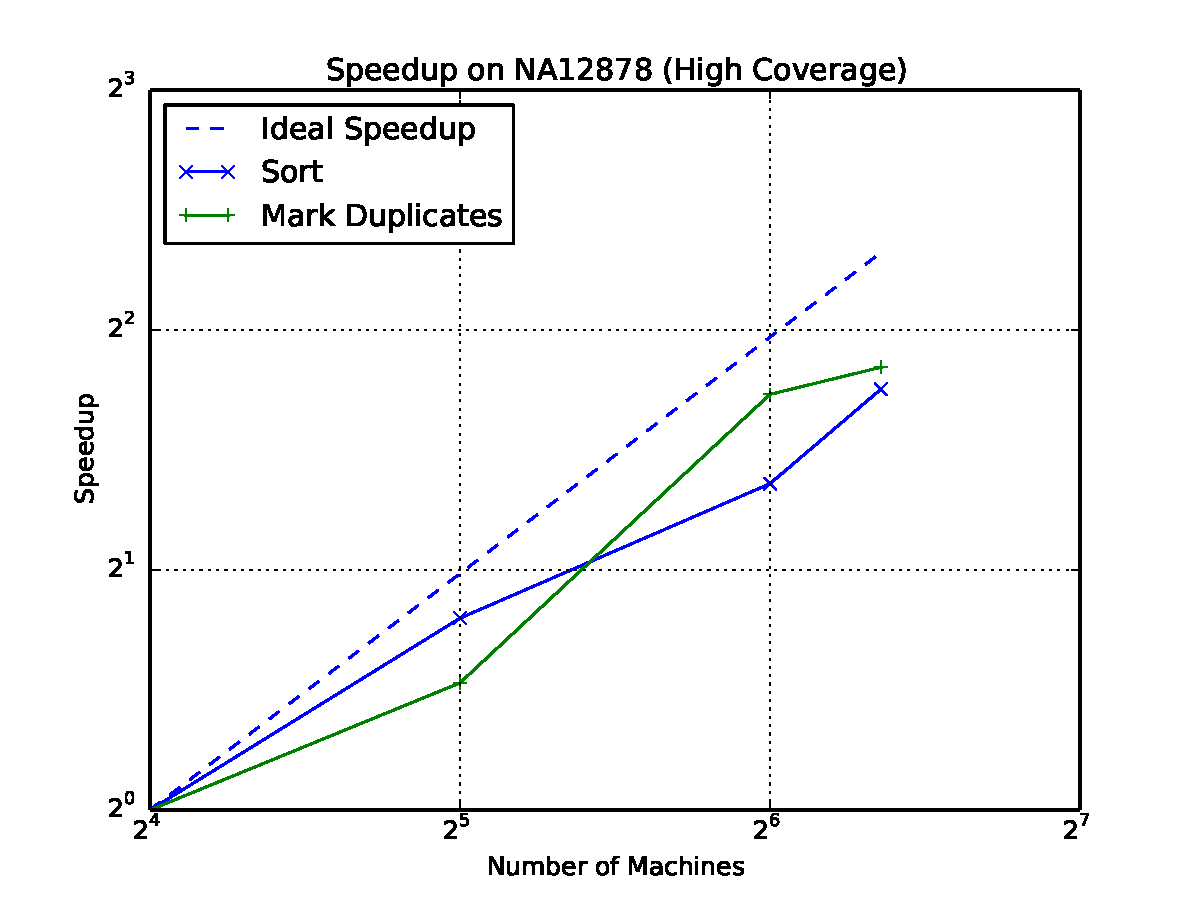
\includegraphics[width=0.99\linewidth]{graphs/speedup_na12878.pdf}
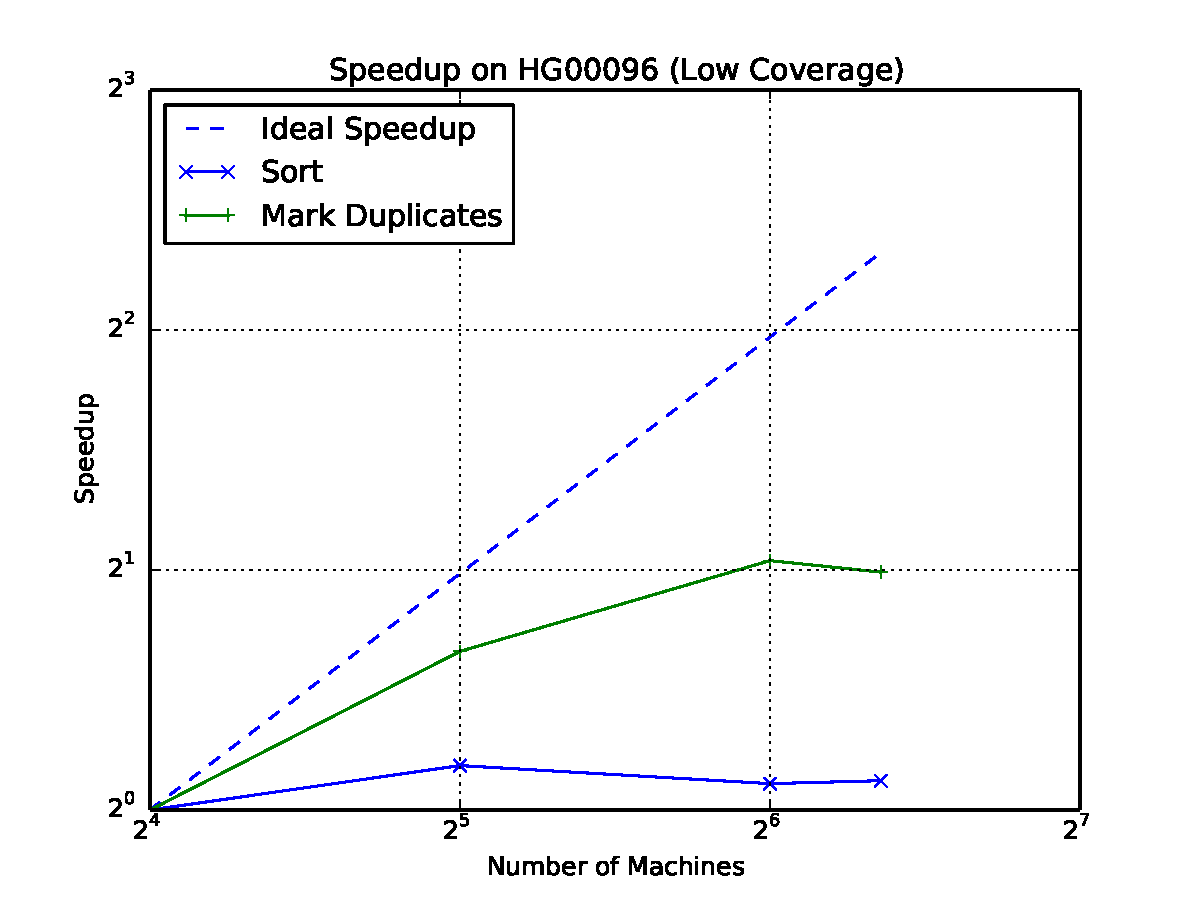
\includegraphics[width=0.99\linewidth]{graphs/speedup_hg00096.pdf}
\end{center}
\caption{Speedup when running \textit{Sort} and \textit{Mark Duplicates} on NA12878 and HG00096}
\label{fig:speedup}
\end{figure}

NA12878 sees linear speedup for both \textit{Sort} and \textit{Mark Duplicates} through 82 nodes. With 82 nodes, it takes 8.8 minutes to sort reads, and 14 minutes to
mark duplicate reads across the 250GB file. HG00096 is a significantly smaller genome at 16 GB. Although the speedup from sorting diminishes after 16 nodes, duplicate
marking sees speedup through 64 nodes. With HG00096 on 64 nodes, each machine in the cluster is responsible for processing only 250MB of data. Sorting completes in
3.3 minutes, and duplicate marking completes in 2.3 minutes. The speedup is limited by several factors:

\begin{itemize}
\item Although columnar stores have very high read performance, they are limited by write performance. Our tests exaggerate this penalty---as a variant calling pipeline will
consume a large read file, but then output a variant call file that is approximately two orders of magnitude smaller, the write penalty will be reduced.
\item Additionally, for large clusters, straggler elimination is an issue. Phases of both \textit{Sort} and \textit{MarkDuplicates} currently suffer from stragglers---we are in
the process of addressing these issues.
\end{itemize}

However, as noted above, speedup continues until we reach approximately 1GB of data per node for sorting, or 250MB of data per node for duplicate marking. For a high
coverage whole genome like NA12878, this should theoretically allow speedup through 250 nodes for sorting and 1,000 nodes for duplicate marking.

\section{Discussion}
\label{sec:discussion}

As a quick reference, Table~\ref{tab:comparison} compares ADAM's read and variant/genotype formats against the BAM and VCF formats.

\begin{table}[h]
\processtable{Comparison of File Formats\label{tab:comparison}}
{\begin{tabular}{ l c c }
\toprule
 & \bf BAM \& VCF & \bf ADAM \\
\midrule
\bf Scalability & $\le$8 machines & $>$100 machines \\
\bf Global Information & Centralized header & Store in all records \\
\bf Cross Platform Support & Implemented via API & Direct record access \\
\midrule
 & \bf BAM & \bf ADAM \\
\midrule
\bf Size & 1.0$\times$ & 0.75-0.9$\times$ \\
\bf Can Query? & Add-on~(GQL) & Natively supported \\ 
\midrule
& \bf VCF & \bf ADAM \\
\midrule
\bf Can Query? & No & Natively supported \\ 
\bf Access subset of samples? & No & Natively supported \\
\bf Annotation Support & Only variant/genotype & User specified \\
\botrule
\end{tabular}}{}
\end{table}

In the remainder of this section, we discuss the evolution of ADAM. First, we discuss how we envision the computing systems that are used in bioinformatics to evolve, and
how ADAM enables this evolution. Finally, we discuss the design decisions and processes that we have incorporated that will make it easy to revise the ADAM data formats.

\subsection{Single Node Processing vs. Dedicated Clusters vs. Cloud Computing}
\label{sec:single-vs-clusters-vs-cloud}

A central goal during the development of ADAM was to not force users to follow specific patterns. As such, we have also made efforts to design the ADAM format and command
line utilities to be portable across different computing installations. We envision that end users will be using ADAM on single workstations, dedicated computing
clusters, or through a cloud computing provider like Amazon EC2, Google Compute Engine, or Microsoft Azure. As can be seen in~\S\ref{sec:performance}, ADAM performs
admirably on all platforms, achieving a 2$\times$ speedup over the current state-of-the-art on a single node, and near-linear speedup when distributed.

As traditional genomics workflows could not easily or efficiently use compute clusters, many users have performed the bulk of their processing on beefy workstations. We predict
that the rise of distributed computing tools for genomics will soon render workstations unattractive. Instead, we expect that clinical/research centers will either process
consistently high volumes of genomic data and build and maintain their own dedicated compute farms, or will use a cloud computing platform for infrequent data processing
needs. The benefits of cloud computing include:

\begin{itemize}
\item Commercial cloud platforms are economically attractive as they do not present any capital acquisition costs, nor do they have maintenance costs.
\item Additionally, cloud platforms tend to offer several levels of service differentiation. Users can trade cost for performance, as the number of machines and performance of
machines can be selected. Additionally, cloud platforms also frequently auction unused slots off at below-market prices~(\emph{spot instances}, which can further reduce costs.
\item System setup can be simplified through the use of systems like \textit{Docker}~\citep{docker} for distributing consistent application images.
\item Inexpensive pay-as-you-go storage solutions are available which provide good performance when used with a cloud service.
\end{itemize}

We anticipate that formats like ADAM will ease this transition, as ADAM can be used efficiently on all platforms. Additionally, ADAM's stack model explicitly allows for significant
flexibility in the format, which will allow ADAM to easily adapt to future computing innovations.

\subsection{Syntax vs. Semantics}
\label{sec:syntax-vs-semantics}

When developing a new genomics file format, it is important to address both the problems of syntax and semantics. A format that is \emph{syntactically good} will be easily
adaptable to multiple platforms, provide good programming abstractions and APIs, and will be performant. A format that is \emph{semantically good} will provide data
representations that closely mirror the biological and algorithmic processes they represent.

The core of the ADAM project is focused on improving the syntax used for representing biological data. Our focus on semantics is limited to introducing semantic improvements
for variant and genotype data that allows for better representation of joint called data and annotations~\S\ref{sec:adamvariant}. However, while we do not address the greater
issues of semantics, we provide a clean platform for tacking these issues because of the ADAM stack and its ability to support broader access and computational patterns.
For example, ADAM data can easily be accessed using relational databases like Shark and Impala~\citep{xin13shark, impala}. Additionally, ADAM can be used as the base
of a graph-based data representation through GraphX~\citep{xin13graphx}. This design decision allows for the easy and clean extension of ADAM's semantics.

\subsection{Evolution of Standard}
\label{sec:evolution-of-standard}

ADAM's read, pileup, variant, and genotype formats are designed to evolve easily. The formats are simple to evolve because they are expressed as an explicit schema
in Avro. Avro allows for an application that has been compiled against a specific version of the schema to read data that has been written in an older or newer version of the
schema, as long as a simple process is followed when updating the schema.

Additionally, we have designed the formats to allow for user defined fields to be added without changing the core schema. Read data uses ``attributes,'' in a fashion similar to
the SAM/BAM format. For variant and genotype data, our variant context implementation~(see~\S\ref{sec:adamvariant}) supports several different and expressive ways for
defining new fields. The variant context method is superior to the annotations provided by the VCF standard, as it provides higher expressivity while promoting better
organization.

ADAM is a community effort, and all members of the greater bioinformatics community are invited to modify both the data formats and the processing pipelines. The ADAM team
has established a Request For Comment~(RFC) system that is similar to the one used by the Internet Engineering Task Force~(IETF). Here, modifications are proposed and
opened for public discussion for a set time frame. After a consensus is reached, the format can be amended. The RFC platform is hosted at our project
website~(\url{http://adam.cs.berkeley.edu/rfc}).

\section{Conclusion}
\label{sec:conclusion}

This paper presents ADAM, a new data storage format and processing pipeline for genomics data. Our reference implementation makes use of efficient columnar storage
systems to improve the lossless compression available for storing read data, and uses in-memory processing techniques to eliminate the read processing bottleneck faced by
modern genomics pipelines. We also present APIs that enhance developer access to read, pileup, genotype, and variant data.

We are currently in the process of extending ADAM to support SQL querying of genomic data, and extending our transformations API to more programming languages. 
ADAM promises to improve the development of applications that process genomic data, by removing current difficulties with the extraction and loading of data and by
providing simple and performant programming abstractions for processing this data at scale.

\section*{Acknowledgement}
\label{sec:acknowledgement}

The authors would like to thank their many colleagues who provided feedback on early implementations of ADAM, and on drafts of the manuscript. Additionally, we would
like to thank Uri Laserson, David Haussler, Adam Novak, Mauricio Carnerio, and Joel Thibault for their feedback on technical direction and format implementation.

\paragraph{Funding\textcolon}
\label{sec:funding}

This research is supported in part by NSF CISE Expeditions award CCF-1139158 and DARPA XData Award FA8750-12-2-0331, a NSF
Graduate Research Fellowship (DGE-1106400) and gifts from Amazon Web Services, Google, SAP,  Apple, Inc., Cisco, Clearstory Data,
Cloudera, Ericsson, Facebook, GameOnTalis, General Electric, Hortonworks, Huawei, Intel, Microsoft, NetApp, Oracle, Samsung, Splunk,
VMware, WANdisco and Yahoo!.

\bibliographystyle{natbib}

\bibliography{adam-ismb-2013}

\end{document}
